\section{Choosing a classical optimizer}
Many classical optimizers have been used within QAOA in literature \cite{blekos_review_2024}. However, we restricted ourselves
to some optimizers that are generally available in the very well-known SciPy Python's library, and tried different types: bounded,
unbounded, gradient-free, and gradient-based. For example, Nelder-Mead showed good performance, but it was discarded due to its bad
scalability with the number of parameters. Cobyla resulted in poor performance due to local minima trapping even for a few-qubit
problems, so it was also discarded. BFGS and L-BFGS-B are two gradient-based optimizers that were found to give the best results:
\begin{itemize}
    \item L-BFGS-B is a bounded optimizer that fits perfectly for QUBO and MaxCut problems. These problems contain symmetries
    that allow us to restrict the variational parameters into specific intervals, and this is the reason why it makes perfect
    sense to use a bounded optimizer in this cases.
    \item BFGS is an unbounded optimizer, i.e. the variational parameters can take any real value. We observed that this method
    outperforms L-BFGS-B in all the tested cases, up to 8--qubit problems. Our feeling is that BFGS is able to avoid some local
    minima in which L-BFGS-B gets trapped thanks to its unbounded nature.
\end{itemize}

\begin{figure}[h]
    \centering
    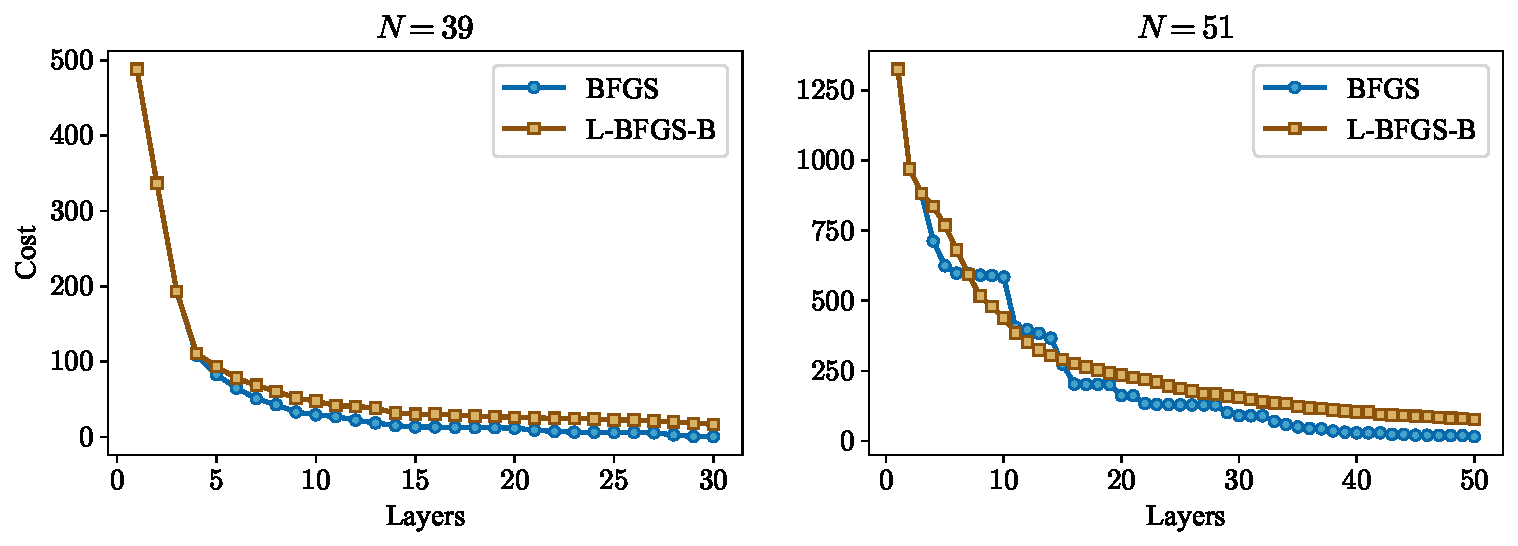
\includegraphics[width=1\textwidth]{03-results/figs/optimizer_comparison.pdf}
    \caption{Cost evolution comparison between BFGS and L-BFGS-B optimizers for factorizing $N=39$ and $N=51$
    using the standard protocol. These problems use 5 and 6 qubits, respectively, but the tendency has been observed
    up to 8-qubit problems.}
    \label{fig:optimizer_comparison}
\end{figure}

Many studies {\color{red} (add references, \cite{zhou_quantum_2020,diez-valle_universal_2025})} show how adiabatic-like passages surge in the
evolution of parameters through the different layers, where typically $\gamma$ --related to interaction field-- tends to start near
zero and increase monotonically until reaching a maximum value, while $\beta$ --related to transversal field-- starts at a maximum
value and decreases monotonically to zero. As shown in Fig.~\ref{fig:optimizer_parameter_comparison}, this behavior arises when
restricting variational parameters within specific intervals.

\begin{figure}[h]
    \centering
    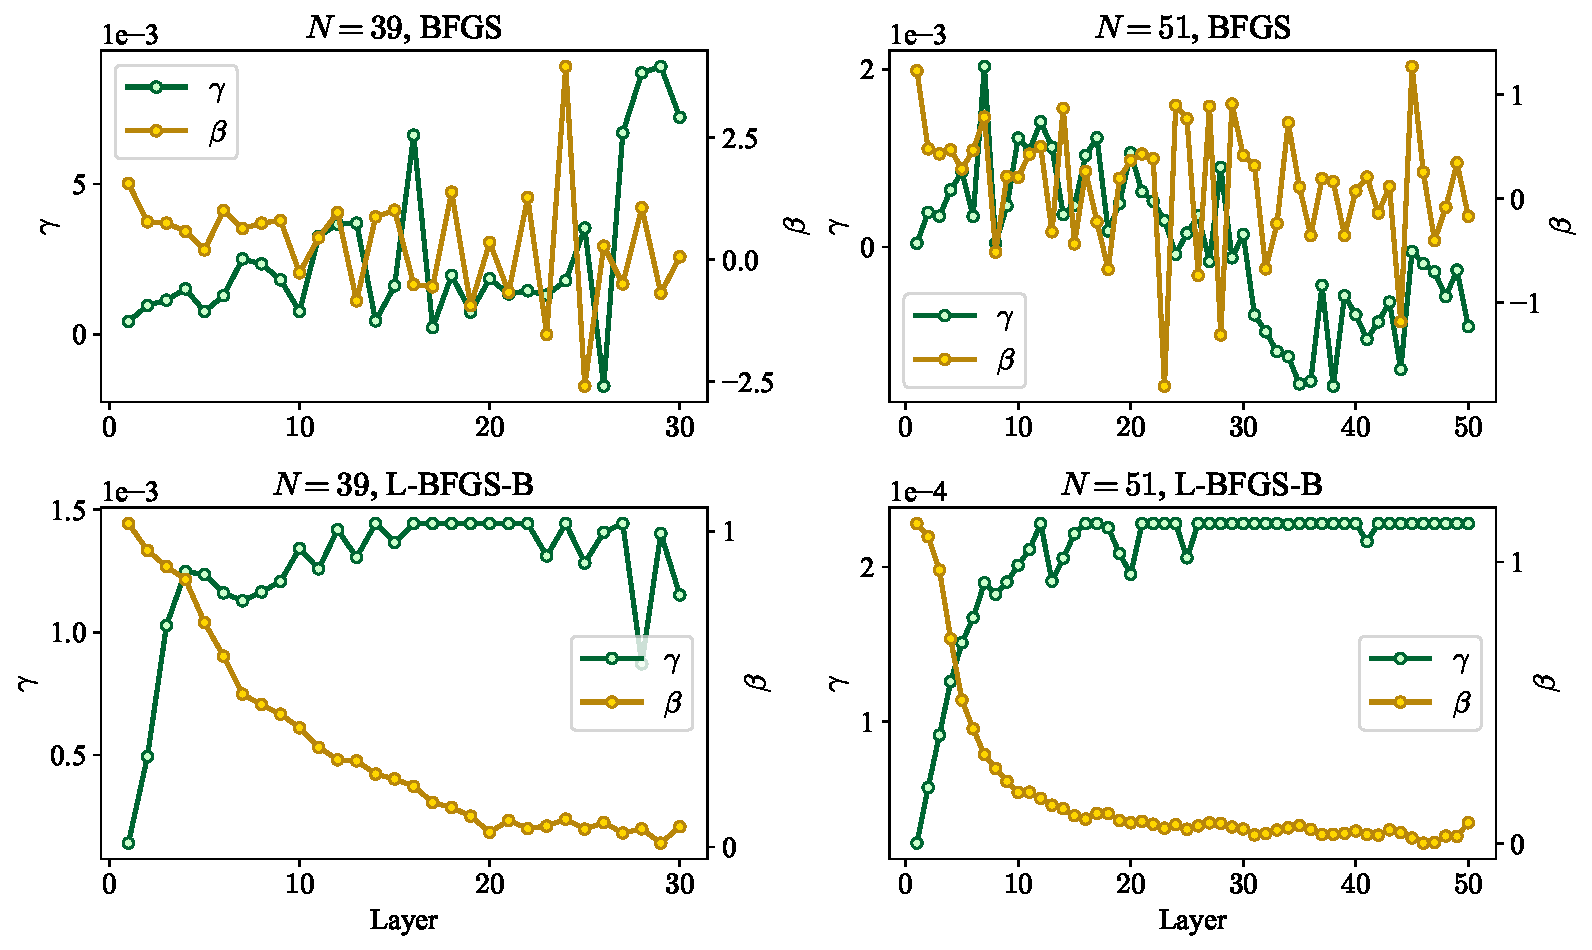
\includegraphics[width=1\textwidth]{03-results/figs/optimizer_parameters_comparison.pdf}
    \caption{Evolution of variational parameters for $N=39$ and $N=51$, using BFGS and L-BFGS-B classical optimizers for
    the standard protocol. Notice the adiabatic-like behavior of $\gamma$ and $\beta$ when using L-BFGS-B.}
    \label{fig:optimizer_parameter_comparison}
\end{figure}